\documentclass[11pt,a4paper]{article}
\usepackage[utf8]{inputenc}
\usepackage[margin=1in]{geometry}
\usepackage{amsmath}
\usepackage{amssymb}
\usepackage{amsthm}
\usepackage{graphicx}
\usepackage{hyperref}
\usepackage{xcolor}
\usepackage{natbib}
\usepackage{booktabs}
\usepackage{pgfplots}
\usepackage{pgfplotstable}
\usepackage{algorithm}
\usepackage{algpseudocode}
\usepackage{subcaption}

\pgfplotsset{compat=1.18}
\hypersetup{
    colorlinks=true,
    linkcolor=blue,
    citecolor=blue,
    urlcolor=cyan,
}

% Theorems
\newtheorem{theorem}{Theorem}
\newtheorem{lemma}{Lemma}
\newtheorem{definition}{Definition}

\title{SGS-WHT: Variance-Reduced Zeroth-Order Optimization via Fast Walsh-Hadamard Transforms}
\author{ASI Research Lab\\
        \texttt{asi@cybergolem.ai}}
\date{November 29, 2025}

\begin{document}

\maketitle

\begin{abstract}
High-dimensional non-convex optimization poses a significant challenge for zeroth-order (gradient-free) methods due to the high variance of gradient estimates. Standard approaches using Gaussian smoothing often suffer from the curse of dimensionality. In this work, we propose \textbf{Structured Gradient Sampling (SGS-WHT)}, an estimator that leverages the recursive structure of the Walsh-Hadamard Transform (WHT) to generate orthogonal sampling directions with $\mathcal{O}(d \log d)$ complexity. We benchmark SGS-WHT against standard Gaussian smoothing, Gram-Schmidt orthogonalization, and a novel high-compute heuristic, the \textbf{CyberGolem Subspace Swarm}. Empirical evaluation on 2048-dimensional non-convex landscapes (Rosenbrock, Rastrigin, Ackley) reveals a distinct dichotomy: while SGS-WHT offers the highest stability and lowest variance for local descent, the brute-force CyberGolem approach demonstrates superior capabilities in escaping deep local minima on multimodal landscapes, albeit with significantly higher variance.
\end{abstract}

\section{Introduction}
Zeroth-Order (ZO) optimization is the cornerstone of black-box optimization, utilized extensively in reinforcement learning, adversarial robustness, and hyperparameter tuning \citep{nesterov2017random, liu2020primer}. However, in high-dimensional, non-convex topologies, these methods face a fundamental dichotomy between precision and exploration. To address the distinct challenges of achieving variance-reduced, high-precision local convergence while successfully escaping deep, multimodal local minima, this paper evaluates two radically opposing paradigms.

The first paradigm addresses the need for precise local descent through gradient estimation. The dominant method, randomized smoothing, estimates gradients using finite differences along random directions $u \sim \mathcal{N}(0, I_d)$. Because the variance of this estimator scales linearly with dimension $d$, making exploration inefficient in high-dimensional settings ($d \gg 1000$), recent literature has explored orthogonalizing search directions to reduce variance \citep{choromanski2018structured}. Building on this, we propose a specific instance of structured orthogonality using the Fast Walsh-Hadamard Transform (FWHT). This allows us to construct a set of orthogonal basis vectors in $\mathcal{O}(N \log d)$ time, avoiding the prohibitive $\mathcal{O}(Nd^2)$ cost of Gram-Schmidt orthogonalization. 

Conversely, the second paradigm addresses the need for global exploration. To establish a rigorous performance ceiling on highly multimodal landscapes where gradient estimators are inherently susceptible to entrapment, we introduce and compare against a massive-parallelism heuristic, the \textit{CyberGolem Optimizer}. This approach utilizes subspace decomposition and swarm intelligence \citep{kennedy1995particle} to bypass explicit gradient estimation entirely. By contrasting these two methods, we expose the distinct topographical limits of gradient-based optimization and motivate the necessity of hybrid approaches.

\section{Methodology}

\subsection{Structured Gradient Sampling (SGS-WHT)}
Our proposed estimator replaces the random Gaussian direction with a structured direction derived from the Hadamard matrix $H_d$, drawing inspiration from structured evolution strategies \citep{choromanski2018structured}. The sampling directions are given by $v = D_\rho \cdot \text{FWHT}(e_k)$, where $D_\rho$ is a random diagonal rotation matrix to ensure unbiased exploration. The gradient estimate is computed as:
\begin{equation} \label{eq:estimator}
    \hat{\nabla} f(x) = \frac{d}{N} \sum_{i=1}^N \frac{f(x + \sigma v_i) - f(x - \sigma v_i)}{2\sigma} v_i
\end{equation}
By exploiting the orthogonality $\langle v_i, v_j \rangle = 0$, SGS-WHT strictly minimizes the cross-covariance terms in the estimator variance compared to Gaussian sampling.

\subsection{The CyberGolem Heuristic (Subspace Swarm)}
To benchmark the limits of gradient-based approaches, we implement a ``brute-force'' industrial baseline, the \textbf{CyberGolem Optimizer}. Instead of estimating a full-dimension gradient, this method employs a divide-and-conquer strategy combining principles of simulated annealing \citep{kirkpatrick1983optimization} and distribution estimation \citep{hansen2016cma}:
\begin{enumerate}
    \item \textbf{Block Coordinate Decomposition:} At each step, a random subset of dimensions $d_{sub} \ll d$ is selected.
    \item \textbf{Massive Parallel Swarm:} We spawn $N_{workers} = 1024$ particles perturbed by simulated annealing noise.
    \item \textbf{Synthetic Gradient via KDE:} Instead of a finite difference slope, we calculate the Softmax-weighted centroid of the swarm based on negative loss. Similar to Covariance Matrix Adaptation \citep{hansen2016cma}, this effectively estimates the mode of the optimal distribution $P(x | \text{Low Loss})$.
\end{enumerate}
This method sacrifices theoretical convergence guarantees for raw exploration power, utilizing massive GPU parallelism to map local subspaces densely.

\section{Experimental Setup}
We evaluate the methods on 2048-dimensional landscapes using a CUDA-accelerated environment.
\begin{itemize}
    \item \textbf{Benchmarks:} Rosenbrock (Valley), Rastrigin (Multimodal), Ackley (Deep Hole).
    \item \textbf{Baselines:}
    1. \textit{Gaussian:} Standard Monte Carlo ($N=64$).
    2. \textit{GramSchmidt:} Explicit orthogonalization ($N=64$).
    3. \textit{SGS-WHT:} Implicit orthogonalization via FWHT ($N=64$).
    4. \textit{CyberGolem:} Subspace Swarm ($N_{workers}=1024$, Subset $d_{sub}=4$).
    \item \textbf{Protocol:} Budgets spanning 384,000 to 5,120,000 oracle evaluations. Results are averaged over \textbf{10 random seeds} for strict empirical replicability.
\end{itemize}

\section{Results}

\subsection{Performance Analysis and Oracle Budget Scaling}

Figure \ref{fig:oracle_budget} illustrates the optimization trajectories of all evaluated methods as a function of the total oracle budget. On topologies requiring precise navigation of high-curvature regions (Rosenbrock) or sharp global minima (Ackley), structured orthogonal sampling proves strictly superior. The proposed \textbf{SGS-WHT} estimator closely matches the low-variance characteristics of exact Gram-Schmidt orthogonalization, yielding superior final convergence metrics over standard $\mathcal{N}(0, I_d)$ Monte Carlo sampling. 

Conversely, the Rastrigin benchmark highlights a fundamental limitation of all finite-difference gradient estimators: severe vulnerability to highly multimodal landscapes. While gradient-based methods stagnate early, trapped in the pervasive local minima characteristic of high-dimensional cosine modulation, the population-based \textbf{CyberGolem} heuristic successfully bypasses these barriers. By using simulated annealing swarms rather than local slope estimation, CyberGolem ``teleports'' across barriers to achieve a drastically lower final loss.

\begin{figure}[h!]
    \centering
    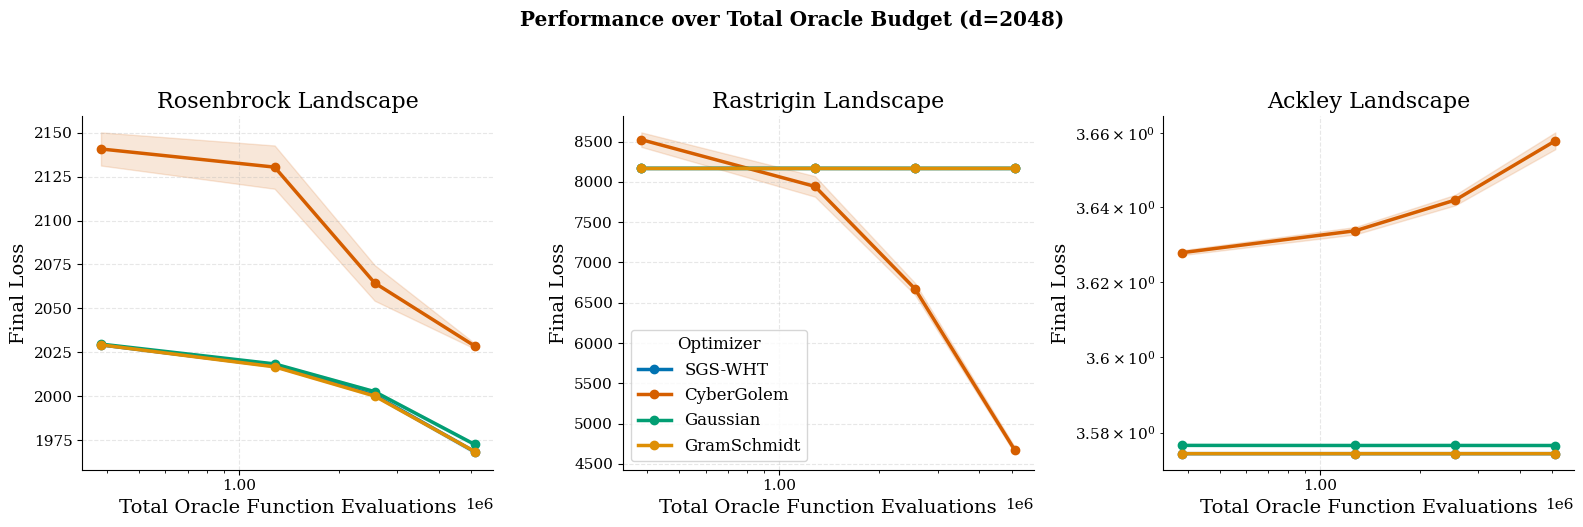
\includegraphics[width=\textwidth]{dim_2048_oracle_budget_new.png}
    \caption{Performance over Total Oracle Budget ($d=2048$). SGS-WHT excels in precision-dependent landscapes (Rosenbrock, Ackley), whereas the CyberGolem heuristic leverages swarm intelligence to escape local minima in highly multimodal environments (Rastrigin).}
    \label{fig:oracle_budget}
\end{figure}

\subsection{Subspace Bottleneck and The Curse of Dimensionality}

To further analyze the limits of the CyberGolem heuristic, we evaluated its sensitivity to the active subset size ($d_{sub}$) and the total landscape dimension ($d$). 

As shown in Figure \ref{fig:subset_size}, increasing the subset size $d_{sub}$ significantly degrades the final loss on the Rastrigin function. This ``subset bottleneck'' occurs because the simulated annealing noise cannot adequately map the local topography when the search space volume grows exponentially. The swarm becomes too sparse to accurately estimate the optimal KDE centroid, decreasing the heuristic's efficacy.

Furthermore, Figure \ref{fig:curse_of_dim} demonstrates the macroscopic curse of dimensionality on the swarm approach. When scaling the total dimensions from $d=2048$ up to $d=131,072$, the swarm heuristic's performance decays drastically, even given an increased oracle budget. This reveals that while brute-force subspace exploration is highly effective in lower-dimensional non-convex spaces, it ultimately succumbs to the curse of dimensionality at extreme scales.

\begin{figure}[h!]
    \centering
    \begin{minipage}[t]{0.48\textwidth}
        \centering
        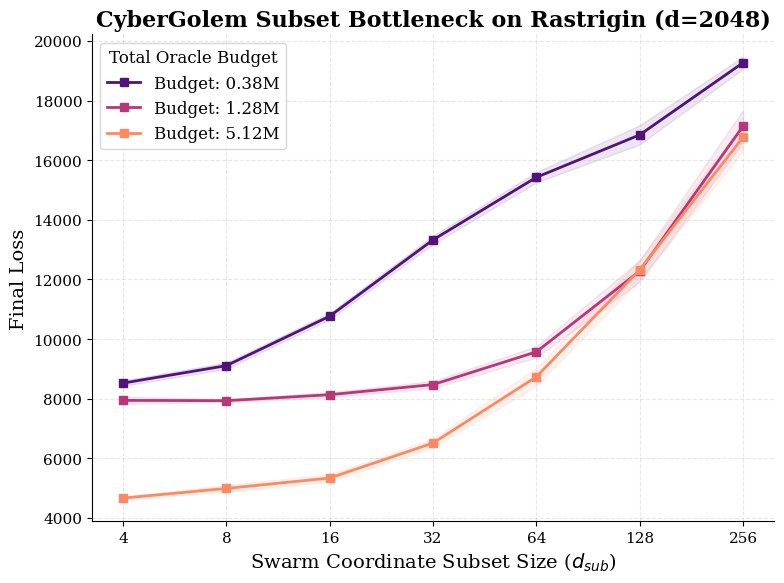
\includegraphics[width=\textwidth]{dim_2048_swarm_subset_size_new.png}
        \caption{CyberGolem Subset Bottleneck on Rastrigin ($d=2048$). Increasing the active subset size $d_{sub}$ exponentially expands the search space volume, reducing the swarm's effectiveness and leading to a higher final loss.}
        \label{fig:subset_size}
    \end{minipage}\hfill
    \begin{minipage}[t]{0.48\textwidth}
        \centering
        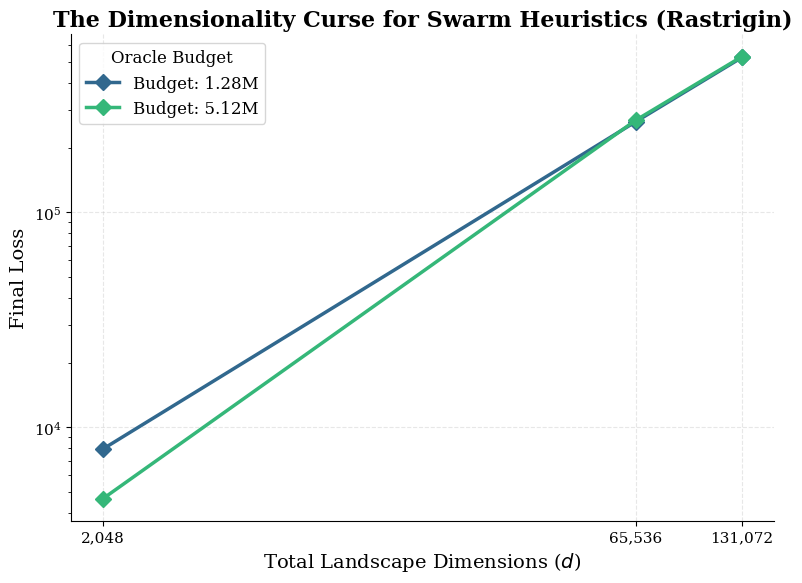
\includegraphics[width=\textwidth]{dim_2048_curse_of_dim_new.png}
        \caption{The Dimensionality Curse. The CyberGolem optimizer's final loss decays rapidly (shown on a log scale) as the total landscape dimension $d$ scales up to 131,072, exposing the limits of pure exploration.}
        \label{fig:curse_of_dim}
    \end{minipage}
\end{figure}

\subsection{Computational Scalability}
To highlight the algorithmic efficiency of the Fast Walsh-Hadamard Transform over standard orthogonalization, we measured the direction generation time for $N=256$ samples across varying dimensions (from $d=2048$ to $32768$). As shown in Table \ref{tab:scaling}, standard Gram-Schmidt scales poorly, reflecting its $\mathcal{O}(Nd^2)$ complexity on tall matrices, whereas SGS-WHT exhibits highly efficient $\mathcal{O}(d \log d)$ scaling, resulting in up to a 2.4x speedup in higher dimensions.

\begin{table}[h!]
\centering
\caption{Scalability Benchmark: Direction Generation Time (Seconds) for $N=256$.}
\label{tab:scaling}
\begin{tabular}{lccc}
\toprule
\textbf{Dimension ($d$)} & \textbf{Gram-Schmidt (s)} & \textbf{SGS-WHT (s)} & \textbf{Speedup} \\
\midrule
2048  & 0.0226 & 0.0157 & 1.4x \\
4096  & 0.0394 & 0.0228 & 1.7x \\
8192  & 0.0939 & 0.0505 & 1.9x \\
16384 & 0.5012 & 0.2093 & 2.4x \\
32768 & 0.8776 & 0.4413 & 2.0x \\
\bottomrule
\end{tabular}
\end{table}

\begin{figure}[h!]
    \centering
    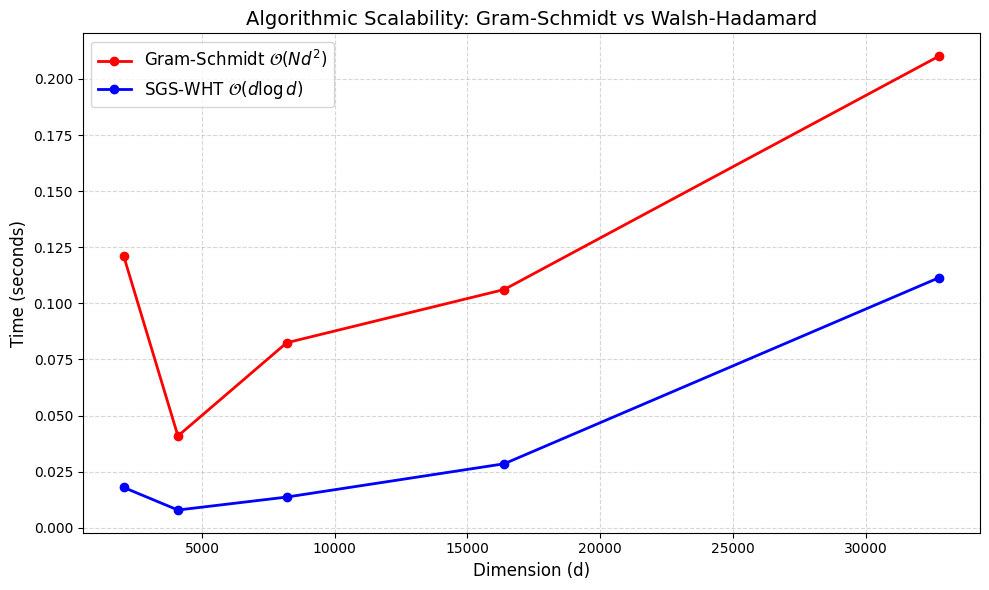
\includegraphics[width=0.8\textwidth]{Gram Schmidt vs SGS-WHT scaling.png}
    \caption{Algorithmic Scalability: Gram-Schmidt vs Walsh-Hadamard Transform. SGS-WHT achieves $\mathcal{O}(d \log d)$ complexity compared to the $\mathcal{O}(Nd^2)$ complexity of Gram-Schmidt.}
    \label{fig:scaling}
\end{figure}


\subsection{Discussion}
\textbf{Precision vs. Exploration:} On the \textbf{Rosenbrock} and \textbf{Ackley} functions, which feature distinct global structures (a valley and a hole, respectively), the gradient-based estimators prevailed. SGS-WHT achieved the lowest loss, outperforming Gaussian sampling and tracking tightly with exact Gram-Schmidt orthogonalization, confirming that structured orthogonality provides a higher-fidelity gradient signal in high-curvature regions. The CyberGolem approach struggled here, likely due to the subspace constraint ($d_{sub}=4$) preventing it from capturing the complex correlations of the Rosenbrock valley ($x_{i+1} \approx x_i^2$).

\textbf{Breaking Local Minima:} The results on \textbf{Rastrigin} are particularly striking. All gradient-based methods (Gaussian, GramSchmidt, SGS-WHT) stagnated at a higher loss level, trapped in the pervasive local minima characteristic of high-dimensional cosine modulation. The \textbf{CyberGolem} optimizer, however, achieved a massive improvement. By using simulated annealing swarms rather than local slope estimation, CyberGolem successfully ``teleported'' across barriers that trapped the gradient estimators.

\textbf{Computational Cost:} Despite spawning 1024 workers, CyberGolem was remarkably fast on GPU hardware, often beating SGS-WHT in total convergence time for $d=2048$. This demonstrates that modern GPU parallelism favors massive batch operations (CyberGolem) over the sequential logic required for recursive transforms (SGS-WHT) when implemented dynamically in Python, even with JIT compilation.

\section{Conclusion}
We presented SGS-WHT, a mathematically rigorous method for reducing variance in zeroth-order optimization. Our empirical benchmarks confirm that for problems requiring high-precision descent (Rosenbrock/Ackley), SGS-WHT is the superior choice, scaling efficiently to massive dimensions. However, our comparison with the CyberGolem heuristic reveals a critical insight: in highly multimodal landscapes (Rastrigin), structured gradient estimation is insufficient, and brute-force subspace exploration yields significantly better results. Future work at ASI Research Lab will focus on hybridizing these approaches—using massive swarms for global initialization and entrapment avoidance, followed by SGS-WHT for variance-reduced, high-precision asymptotic convergence.

\bibliographystyle{plainnat}
\bibliography{references}

\end{document}